\documentclass[unicode, notheorems]{beamer}

% If you have more than three sections or more than three subsections in at least one section,
% you might want to use the [compress] switch. In this case, only the current (sub-) section
% is displayed in the header and not the full overview.
\mode<presentation>
{
  \usetheme[numbers, totalnumbers,nonav]{Statmod}
  \useoutertheme{default}
  \setbeamercovered{transparent}
  \setbeameroption{show notes}
  % \setbeamertemplate{note page}[plain]
}
\usepackage[style=authoryear]{biblatex}
\addbibresource{../biblio-u.bib}

\usepackage[T2A]{fontenc}
\usepackage[utf8]{inputenc}
\usepackage[russian]{babel}
\usepackage{amsthm}
\usepackage{amssymb}
\usepackage{amsthm}
\usepackage{mathtools}
\usepackage{nicefrac}
\usepackage[noend]{algorithm2e}
\usepackage{ragged2e}

\usepackage{graphicx}
\graphicspath{ {../media/} }
\usepackage{epstopdf}
\newcommand{\textitem}[1]{\setbeamercolor{item}{fg=black}\item #1} 

\newtheorem{theorem}{Теорема}
\newtheorem{example}{Пример}
\newtheorem{definition}{Определение}
\newcommand{\E}{\mathrm{E}}
\newcommand{\vfi}{\varphi}
\newcommand{\prob}[1]{\mathsf{P}\left(#1\right)}
\newcommand{\R}{\ensuremath{\mathbb{R}}}
\newcommand{\Tau}{\ensuremath{\mathcal{T}}}
\newcommand{\GothB}{\mathfrak{B}}
\newcommand{\norm}[1]{\left\lVert#1\right\rVert}
\newcommand{\abs}[1]{\left\lvert#1\right\rvert}
\newcommand{\Vhat}{\hat{V}}
\newcommand{\vhat}{\hat{v}}
\newcommand{\maxset}[1]{\max\left\lbrace#1\right\rbrace}
\DeclareMathOperator*{\argmax}{arg\,max}
\DeclareMathOperator*{\argmin}{arg\,min}

% \usepackage{tikz}
% \usetikzlibrary{arrows}
% \usetikzlibrary{positioning}
% \usetikzlibrary{graphs}

\title[Оценки американских опционов]{Имитационная модель американских опционов}

\author[Анастасия Миллер]{Анастасия Александровна Миллер, 622 группа}
\institute[СПбГУ]{Санкт-Петербургский государственный университет \\
    Математико-механический факультет \\
    Кафедра статистического моделирования \\
    \vspace{0.4cm}
    Научный руководитель: д.\,ф.-м.\,н.~Ермаков~С.\,М. \\
    Рецензент: нач.\,лаб.~Дмитриев~А.\,В.
    \vspace{0.3cm}
}
\date[\today]{
    Санкт-Петербург\\
    \today
}

\begin{document}

\begin{frame}
    \titlepage
\end{frame}

\begin{frame}
\frametitle{Что такое опцион} 
\begin{block}{Опцион}
  Договор, по которому потенциальный покупатель или продавец актива получает право, но не обязательство, совершить покупку или продажу данного актива по заранее оговорённой цене в определённый договором момент в будущем или на протяжении определённого отрезка времени.
  \end{block}
  \note{Понятно, что, например, для случая покупки, если определённая договором цена меньше текущей цены на рынке, то реализация этого права даёт некоторый \emph{выигрыш} в деньгах (ровно на разницу между рыночной ценой и ценой из договора). Тогда, согласно концепции безарбитражности, за обретение этого права нужно заплатить, причём столько, чтобы в среднем прибыль и продавца, и покупателя составляла 0.}

  $\Tau$ -- множество моментов, в которые можно \emph{исполнить опцион} (реализовать право на покупку/продажу).\\[10pt]

  \begin{columns}
    \column{0.4\textwidth}
      \emph{Европейский} опцион\\$\Tau = \left\lbrace t \right\rbrace$

    \column{0.4\textwidth}
      \emph{Американский} опцион\\$\Tau = \left[ 0; T \right]$
  \end{columns}
\end{frame}

\begin{frame}
  \frametitle{Математическая модель оценки стоимости опциона} 
   \begin{itemize}
    \item Cостояние базового актива описывается марковским случайным процессом $X_t \in \R^d, t\in{\left[0;T\right]}$, начальное состояние которого фиксировани ($X_0 = \mathrm{const}$).
    \item $h_t(X_t)$ -- дисконтированное значение выигрыша, получаемого при исполнении опциона в момент $t$.
    \item В этих обозначениях в модели эффективного рынка стоимость опциона -- это $$V = \sup_{\tau\in\Tau} \E\left[h_t(X_t)\right].$$
  \end{itemize}

  Для подсчёта $V$ методом моделирования осуществляется переход к дискретному времени (конечному множеству $\Tau$, $\#\Tau = m$).
\end{frame}
\note{Таким образом, для того, чтобы подсчитывать Американский опцион, я нуждаюсь в каждый момент времени в достаточном количестве реализаций случайного процесса $X_t$ для того, чтобы можно было оценить математическое ожидание. Наиболее распространёнными методами решения этой задачи являются метод случайных деревьев, метод сеток и метод линейной регрессии. Метод сеток и метод регрессии тесно связаны между собой, поэтому я буду рассматривать в основном метод линейной регрессии.}

\begin{frame}[t]\frametitle{Оценка по методу случайных деревьев}
В статье \cite{Broadie1997} построены оценки сверху и снизу для стоимости опциона $V$. Для оценки сверху $\Vhat^{RT}(b)$ доказано, что $$\begin{aligned}\forall\;b\in\mathbb N \quad &\E\Vhat^{RT}(b) = V^{RT}(b) \geq V, \\ &\lim_{b\to\infty}V^{RT}(b) = V.\end{aligned}$$
    \begin{figure}
      \centering
      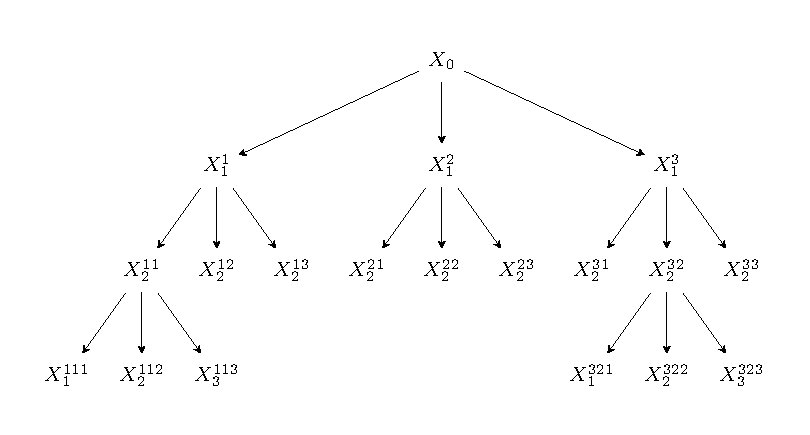
\includegraphics[height=0.4\paperheight]{random_tree}
      \caption{Схема метода для $b=3$}
      \label{fig:random_tree}
    \end{figure}
\note[item]{Чтобы получить достаточное количество реализаций на каждом шаге, используется ветвление. Схема метода, предложенного в статье <<Оценка ценных бумаг Американского типа с помощью моделирования>>, представлена на слайде.} 

\note[item]{Согласно этому методу, из \emph{текущего} состояния базового актива каждый раз моделируются $b$ состояний в \emph{следующий} момент времени, после чего процесс повторяется для каждого из вновь полученных состояний. Для состояний на момент $T$ стоимость опциона, если он не был исполнен до этого момента, известна -- она равна прибыли от исполнения опциона прямо сейчас. Для каждого состояния в каждый из предыдущих моментов времени стоимость равна максимуму из прибыли от исполнения опциона \emph{прямо сейчас} и \emph{матожиданию} прибыли, если сейчас опцион \emph{не} исполнять. Матожидание же оценивается по $b$ реализациям процесса.} 

\end{frame}

\note{Временная сложность алгоритма имеет порядок $b$ в степени числа моментов исполнения. Поэтому такая оценка применяется для небольшого числа моментов исполнения. Обычно оценка считается методом Монте-Карло. Одной из задач моей работы являлось посмотреть, даёт ли использование квази Монте-Карло или рандомизованного квази Монте-Карло какие-то преимущества.}

\begin{frame}[t]\frametitle{Квази Монте-Карло}
    
Квази Монте-Карло последовательности (\cite{sobol}) --- это детерминированные последовательности $\left(x_i\right)_{i\in\mathbb N}$, обладающие улучшенными по сравнению с Монте-Карло свойствами равномерности. \\[10pt]

\begin{tabular}{rcc}
&обычный Монте-Карло&квази Монте-Карло\\
\parbox{3 cm}{ошибка оценки по $N$ испытаниям}&$\displaystyle{O(1 / \sqrt N)}$&$\displaystyle{O(\frac{\left(\ln N\right)^d}{N}})$
\end{tabular}\\[10pt]
\note[item]{Вследствие этого ошибка при оценке величины интеграла с использованием квази Монте-Карло последовательностей убывает быстрее, чем ошибка для классического Монте-Карло} 

\begin{itemize}
  \item В квази Монте-Карло нет процедуры оценки погрешности.\note[item]{В квази Монте-Карло нет процедуры оценки погрешности. Для получения такой процедуры предлагается техника рандомизации квази Монте-Карло.}
   \item Для использования Монте-Карло последовательности необходимо заранее зафиксировать размерность используемых квазислучайных чисел. \note[item]{При этом размерность должна быть равно конструктивной размерности алгоритма, то есть  числу случайных чисел, необходимых для получения одной реализации оценки.}
 \end{itemize} 
\end{frame}

\begin{frame}[t]\frametitle{Рандомизация квази Монте-Карло}

\begin{tabular}{rl}
$\left(x_i\right)_{i\in\mathbb N}$ & \parbox{0.8\textwidth}{квази Монте-Карло последовательность в ${[0;1]^d}$. }\\[10pt]
$\left(\xi_i\right)_{i\in\mathbb N}$ & \parbox{0.8\textwidth}{последовательность случайных величин, равномерно распределённых в ${[0;1]^d}$. }\\[10pt]
$G\in\mathbb N$ & размер группы.
\end{tabular}\\[10pt]

\note[item]{Рандомизация сдвигом заключается в следующем. Квази Монте-Карло последовательность делят на группы, после чего к каждой группе прибавляют по модулю единицы реализацию независимой случайной величины.} 

Рандомизированная квази Монте-Карло последовательность $\left(\tilde{x}_i\right)_{i\in\mathbb N}$:
$$\tilde{x}_{kG + j} = x_{kG + j} + \xi_k \mod 1. $$

Оценка дисперсии оценки $\hat V = \frac{1}{NG}\sum_{i=1}^{NG} \hat V(\tilde{x}_i)$:
$$
\Vhat_{k} = \frac{1}{G}\sum_{j=1}^G \Vhat(\tilde x _{kG + j}), \qquad\mathrm{Var}\Vhat = \frac{1}{N}\sum_{k=1}^N \left(\Vhat- \Vhat_k\right)^2.
$$
% При сравнении с классическим Монте-Карло в классическом методе также используются оценки межгрупповой дисперсии
\note[item]{Тогда внутри группы все точки последовательности оказываются одинаково распределёнными, но всё ещё зависимыми, а вот внутригрупповые средние уже являются независимыми одинаково распределёнными случайными величинами, дисперсию которых можно оценить стандартным способом.% Важно отметить, что при сравнении дисперсии с дисперсией обычного Монте-Карло процедура оценки должна совпадать для рандомизированного квази Монте-Карло и обычного Монте-Карло. То есть последовательность из независимых одинаково распределённых наблюдений точно так же делится на группы и оценивается межгрупповое отклонение.
} 

\end{frame}

\begin{frame}[t]\frametitle{Сравнение оценок для $V^{RT}(b)$}
\note{Давайте же посмотрим, как ведут себя классический, квази и рандомизированный квази Монте-Карло в задаче вычисления оценки по случайным деревьям. Здесь и далее будут использоваться аббревиатуры, обозначенные в верхней чести слайда.} 

\begin{tabular}{rl}
MC & \parbox{0.8\textwidth}{классический метод Монте-Карло}\\
QMC & \parbox{0.8\textwidth}{квази Монте-Карло}\\
RQMC & \parbox{0.8\textwidth}{рандомизированный квази Монте-Карло}
\end{tabular}

\begin{table}
  \caption{Качество оценок $V^{RT}(b)$ с использованием различных последовательностей}
  \label{tab:random_tree}
  \centering

  \begin{tabular}{rrrrrrr}
  тип&$\Vhat^{RT}(b)$&$\mathrm{sd}\Vhat^{RT}(b)$&$\Vhat^{RT}(b) - V^{RT}(b)$\\\hline
  MC&11.232&1.456&0.007\\[2pt]
  QMC Соболя&11.267&-&0.042\\
  RQMC Соболя&11.275&\textcolor{beamer@blendedblue}{0.801}&0.052\\[2pt]
  QMC Холтона&11.267&-&0.042\\
  RQMC Холтона&11.273&1.969&0.050\\[2pt]
  \end{tabular}

   \linespread{0.7}\footnotesize Число ветвей $b=2$, опцион на покупку на 2 актива $X_t = (S^{(1)}_t, S^{(2)}_t)$ с начальной стоимостью $S^{(1)}_0 = S^{(2)}_0 = 100$, ценой из контракта $K = 100$ и функцией выплат $h_t(X_t) = (\max\{S^{(1)}_t, S^{(2)}_t\} - K)^+$. Число моментов исполнения $\#\Tau = 4$.
\end{table}

\end{frame}

\begin{frame}[t]\frametitle{Метод линейной регрессии}
\note{
Следующая часть моей работы заключалась в рассмотрении метода линейной регрессии, о котором я уже упоминала в начале своего рассказа. В методе случайных деревьев математическое ожидание стоимости удержания опциона оценивается с помощью ветвления в каждой точке, где нужна такая оценка. Здесь же строится приближение самой функции условного матожидания.  

Схема метода представлена на слайде. Сначала моделируются несколько траекторий поведения базового актива. Стоимость опциона в конечных точках траекторий известна. Так как стоимость опциона в следующей точке траектории -- это стоимость его удержания на предыдущей точке траектории, по множеству промоделированных траекторий можно оценить зависимость. 
} 
    Предложен в статье \cite{Longstaff2001}. Строится оценка $\Vhat^{LS}(b)$ стоимости Американского опциона, где $b$ -- ширина сетки. Доказано, что $$\Vhat^{LS}(b) \leq V, \quad \Vhat^{LS}(b) \underset{b \to \infty}{\overset{\mathbb P}{\to}} V.$$
\begin{figure}
  \centering
  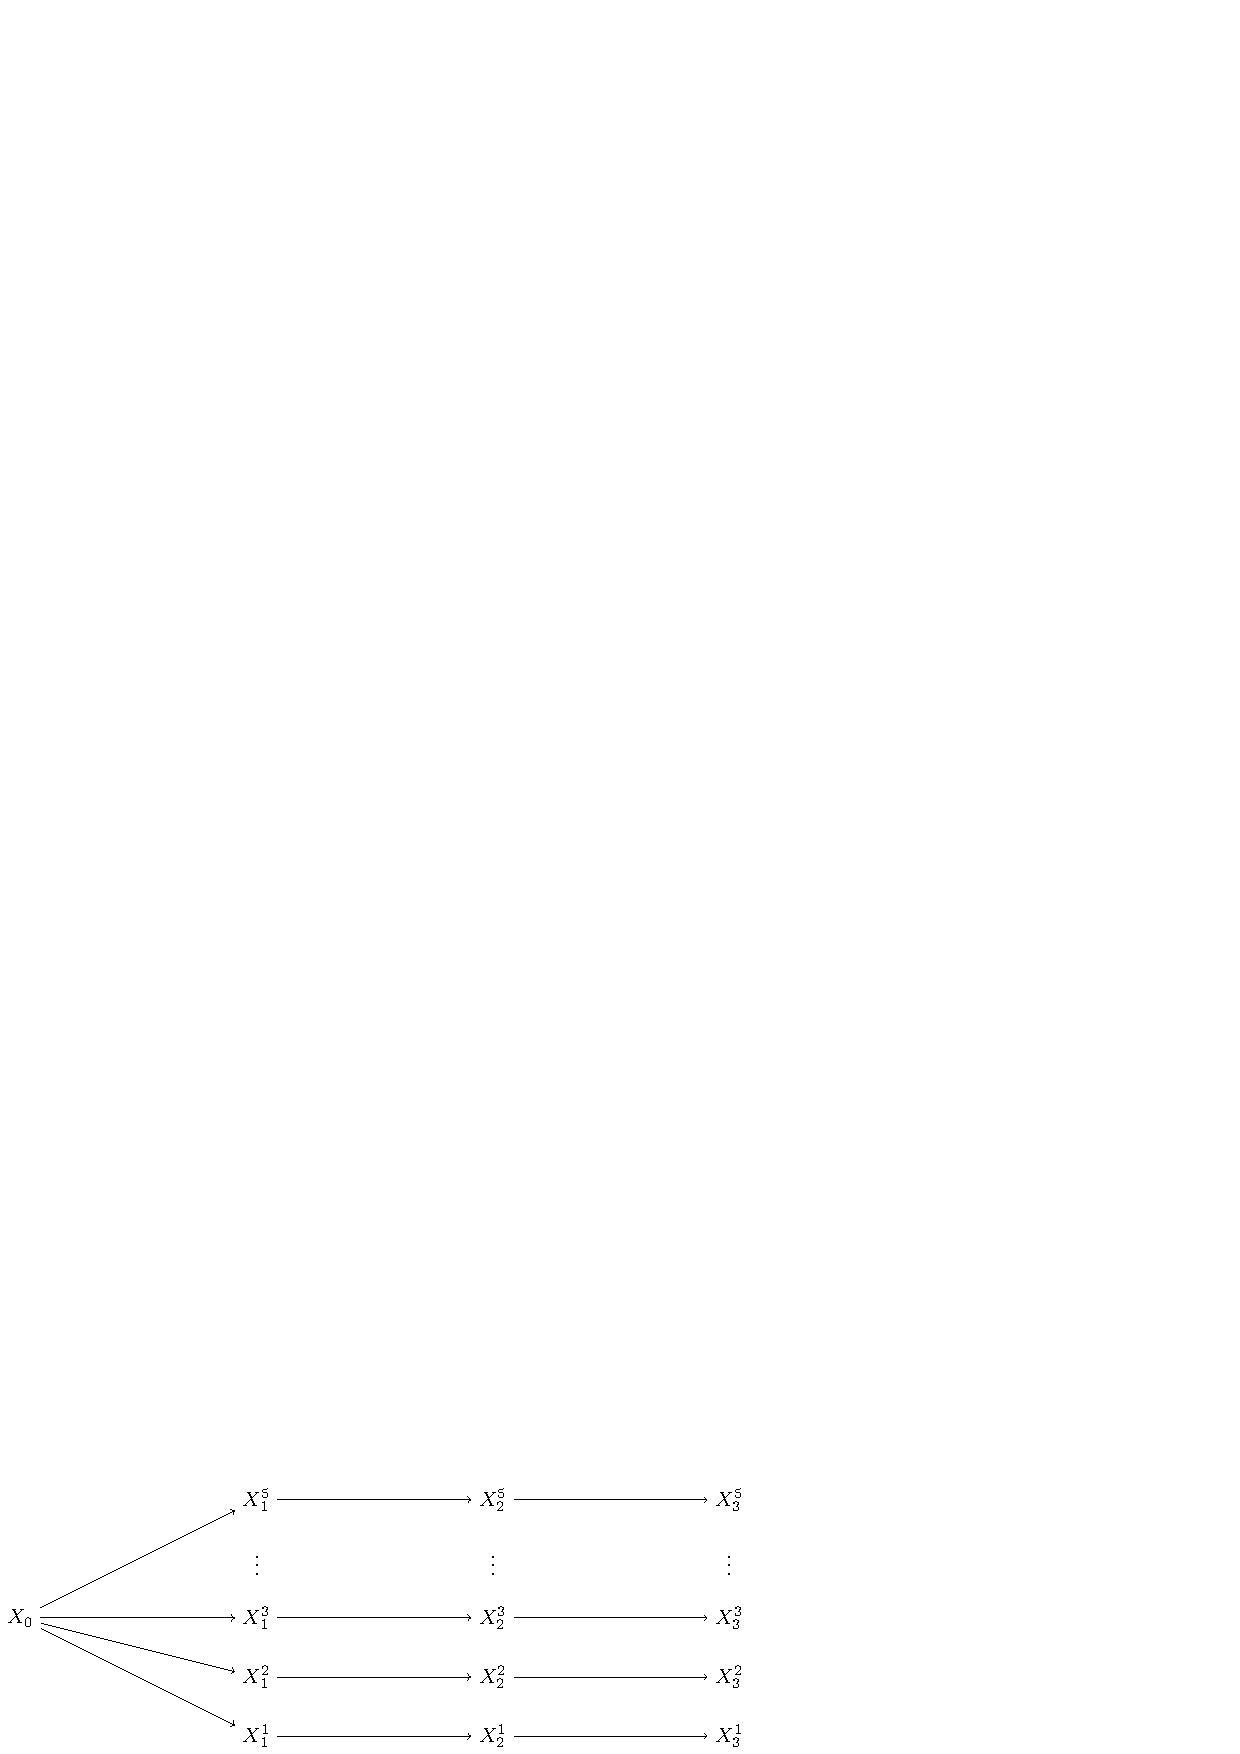
\includegraphics[width=0.9\textwidth]{stohastic_mesh_vector_phase_0.pdf}
  \caption{Схема метода для $\#\Tau = 4$ и $b = 5$}
  \label{fig:lsm}
\end{figure}

\end{frame}

\note{
В оригинальной статье для оценки зависимости предлагается линейная по параметрам регрессия с многочленами Лагера от точек траектории в качестве предикторов, но авторы предполагают, что другие методы оценки условного матожидания тоже могут быть использованы.

Построенные таким образом оценки сходятся по вероятности к истинному значению стоимости опциона.

  Для метода линейной регрессии были проведены эксперименты, аналогичные продемонстрированным для метода случайных деревьев, и показавшие такие же результаты: быстрее всего к математическому ожиданию оценки сходится среднее по отрезкам квазислучайной последовательности Соболя, наименьшая дисперсия у рандомизированной квазислучайной последовательности Соболя, последовательность Холтона удовлетворительных результатов не даёт.
} 

\begin{frame}[t]\frametitle{Метод сглаженных деревьев}
    
\note{
В моей работе предлагается подход, сочетающий в себе метод линейной регрессии и метод случайных деревьев. Схему вы можете видеть на слайде. 

Основная идея заключается в том, чтобы, как только число вершин деревьев на некотором шаге становится слишком большим, заменить во всех этих вершинах оценку выгоды при удержании опциона, получаемую с помощью дальнейшего ветвления, на оценку, получаемую с помощью линейной по параметрам аппроксимации . 

Естественная постановка предполагает, что точки, по которым строится аппроксимация, являются вершинами деревьев, как на картинке. Но оптимальная по памяти реализация алгоритма предполагает, что точки роста (потому что из них вырастает следующее поколение деревьев) выбираются из пространства возможных на этом шаге состояний случайным образом.
} 
\begin{columns}

\column{0.55\textwidth}
Предлагаемая оценка $V^{PT}(b, n, h)$ асимптотически состоятельная и асимптотически несмещённая при $b\to\infty$ и $n\to\infty$.

\column{0.4\textwidth}
Параметры:
\begin{tabular}{rl}
$b$ & \parbox{0.8\textwidth}{\linespread{0.5}\selectfont количество ветвей в дереве}\\[2pt]
$n$ & \parbox{0.8\textwidth}{\linespread{0.5}\selectfont число точек, по которым строится оценка стоимости удержания опциона}\\[6pt]
$h$ & \parbox{0.8\textwidth}{\linespread{0.5}\selectfont высота деревьев}
\end{tabular}

\end{columns}

\begin{figure}[]
  \centering
  \includegraphics[height=0.45\paperheight]{pruned_tree_talk.pdf}
  \caption{Схема метода}
  \label{fig:pruned_tree}
\end{figure}

\end{frame}

\begin{frame}[t]\frametitle{Сравнение метода сглаженных деревьев с методом линейной регрессии}
% написать среднее, дисперсию  и смещение относительно матожидания оценки
    \begin{figure}
    \includegraphics[height=0.5\paperheight]{LSM_vs_pruned_variance_talk.eps} 
    \caption{Дисперсия оценок методов сглаженного дерева и наименьших квадратов для $m = 22$ и одинаковой конструктивной размерности алгоритмов}
  \end{figure}
  \note{Численные эксперименты показали, что дисперсия оценки методом сглаженного дерева существенно ниже, чем дисперсия оценки по методу наименьших квадратов.} 
\end{frame}


\begin{frame}[t]\frametitle{Применение квази Монте-Карло к методу сглаженных деревьев}
    
    \begin{table}
      \caption{Оценки $\Vhat^{PT}$ с использованием различных последовательностей}
      \label{tab:qmc_pruned_tree}
      \centering
    
      \begin{tabular}{rrrrrrrrr}
      $b$&$h$&$n$&тип&$\Vhat$&$\mathrm{sd}\Vhat$&$\mathrm{se}\Vhat$&$\mathrm{bias}\Vhat$\\\hline
      14&2&200&MC&13.379&0.208&3.748&3.742\\
      14&2&200&QMC grid&\textcolor{beamer@blendedblue}{11.632}&-&-&1.995\\
      14&2&200&RQMC grid&13.426&0.893&3.893&3.789\\
      \end{tabular}
    \end{table}

\end{frame}
\note{
  Наиболее естественным способом применить квази Монте-Карло в этом методе является использование его для выбора точек роста. Более того, из-за того, что конструктивная размерность алгоритма при увеличении числа моментов исполнения опциона растёт соответственно, это ещё и практически единственный способ. Ещё теоретически перспективным вариантом является использование квази Монте-Карло размерности, равной конструктивной размерности одного дерева, но численные эксперименты здесь показали неудовлетворительные результаты.

  Интересным моментом здесь является то, что улучшение равномерности сетки, используемой для аппроксимации, в случае метода квази Монте-Карло уменьшает смещение оценки вверх
} 

\begin{frame}[t]\frametitle{Выводы}
    
\begin{itemize}
  \item В существующих алгоритмах оценки стоимости Американского опциона с помощью моделирования возможно применение метода квази Монте-Карло и рандомизованного квази Монте-Карло при условии соблюдения требования на конструктивную размерность алгоритма.
  % \item Предложенный модифицированный метод показал хорошие результаты и без квази Монте-Карло, и с применением квази Монте-Карло.
  \item Предложенный модифицированный метод показал снижение дисперсии в 4.6 раз относительно метода наименьших квадратов с использованием MC. Применение QMC в этой задаче позволило уменьшить смещение построенной оценки относительно истинной стоимости опциона.
\end{itemize}

\end{frame}

\begin{frame}[c]
\frametitle{  }
    
\centering
Вопросы

\end{frame}

\end{document}